\section{Grover's Algorithm}
Grover's search algorithm\cite{grover} is an important quantum algorithm that provides an edge over all classical algorithms in database search. Grover's algorithm shall form the backbone for our search for the nonce. The algorithm uses repeated iterations of a quantum oracle (an oracle stands for a special function) and a diffuser on a superposition of $\ket{0}$ and $\ket{1}$.
\subsection{Oracle}
The oracle is the function that "marks" the states which are the successful search results by applying a negative sign on it. Consider the state $\ket{\omega}$ to be successful. Denote the oracle by $U_\omega$ so that
\begin{equation}
\label{eq:5.1}
U_\omega\ket{x}=
\begin{cases}
\ket{x}&x\neq\omega\\
-\ket{x}&x=\omega
\end{cases}
\end{equation}
The purpose of the oracle is to reflect the coefficient of "solution state ket" about 0, keeping the other coefficients intact. This will help the diffuser amplify amplitudes.
\subsection{Diffuser}
The diffuser is the key component of the Grover Search algorithm. The diffuser amplifies the amplitude of the solution states. It does this by reflecting the amplitudes of the states about the average amplitude. We denote the diffuser by $U_s$, so that
\begin{equation}
\label{eq:5.2}
U_s=2\ket{s}\bra{s}-\mathbb{I}
\end{equation}
where $\ket{s}$ is some arbitrary state.
This is indeed a reflection about the state $\ket{s}$. This is because any arbitrary state $\ket{\psi}$ can be written as $\ket{\psi}=\cos\alpha\ket{s}+\sin\alpha\ket{s_\perp}$ where $\ket{s_\perp}$ is orthogonal to $\ket{s}$. Then we have
\begin{equation}
\label{eq:5.3}
\begin{split}
U_s\ket{\psi}&=U_s\left(\cos\alpha\ket{s}+\sin\alpha\ket{s_\perp}\right)\\
&=\left(2\ket{s}\bra{s}-\mathbb{I}\right)\left(\cos\alpha\ket{s}+\sin\alpha\ket{s_\perp}\right)\\
&=\cos\alpha\left(2\ket{s}\bra{s}\ket{s}-\ket{s}\right)+\sin\alpha\left(2\ket{s_\perp}\bra{s_\perp}\ket{s_\perp}-\ket{s_\perp}\right)\\
&=\cos\alpha\left(2\ket{s}-\ket{s}\right)+\sin\alpha\left(-\ket{s_\perp}\right)\\
&=\cos\alpha\ket{s}-\sin\alpha\ket{s_\perp}
\end{split}
\end{equation}
and we can clearly see that this is a reflection about the $\ket{s}$ axis.


Note that we can write $\ket{s}$ as a sum of two components, one linear function of $\ket{\omega}$ and the other a linear function of a state $\ket{s\prime}$ orthogonal to $\ket{\omega}$. Thus
\begin{equation}
\label{eq:5.4}
\ket{s}=\sin\theta\ket{\omega}+\cos\theta\ket{s\prime}
\end{equation}
Each iteration will comprise $U_s U_{\omega}$, i.e., reflection of $\ket{s}$ about $\ket{s\prime}$ followed by reflection about $\ket{s}$. This results in amplitude amplification. 

\subsection{The Method}
\noindent The method of applying Grover's Search is quite simple.
\begin{enumerate}
\item Initialize $\ket{s}=\bfrac{\ket{0}+\ket{1}}{2}$.
\item Perform $U_{\omega}$ on the state to reflect component along $\ket{\omega}$, keeping components orthogonal to $\ket{\omega}$ intact.
\item Apply $U_{s}$ on this state to reflect the state about $\ket{s}$
\item Repeat steps $2$ and $3$ till search is complete.
\end{enumerate}
The above steps are illustrated in %figure.\\
Now will we actually implement the oracle and the diffuser using quantum logic gates. First let us take a look at the oracle.
\subsubsection*{Implementation of the Oracle}
The oracle is implemented using a phase kickback mechanism. Consider the CNOT gate in \ref{Fig:5.1}. The CNOT gate acts as shown below.
\begin{equation}
\label{eq:5.5}
\begin{split}
&CX\ket{00}=\ket{00}\\
&CX\ket{01}=\ket{01}\\
&CX\ket{10}=\ket{11}\\
&CX\ket{11}=\ket{10}\\
\end{split}
\end{equation}
\begin{figure}[!htb]
   \begin{minipage}{\textwidth}
     \centering
     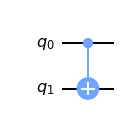
\includegraphics[scale=1]{fig05.01.png}
     \caption{CNOT gate}
     \label{Fig:5.1}
   \end{minipage}
\end{figure}

Now, if we have our classical function $f$ behaving as 
\begin{equation}
\label{eq:5.6}
\begin{split}
f(\omega)&=1\\
f(s)&=0\quad\forall s\neq\omega
\end{split}
\end{equation}
Then we can set up an output qubit as
$$
\ket{out}=\ket{-}=\bfrac{\ket{0}+\ket{1}}{\sqrt{2}}
$$
so that
\begin{equation}
\label{eq:5.7}
CX\ket{f(x)\ out}=
\begin{cases}
\ket{f(x)\ out}&f(x)=0\\
-\ket{f(x)\ out}&f(x)=1
\end{cases}
\end{equation}
Thus we get our oracle. The oracle circuit is shown in \ref{Fig:5.2}. 
\begin{figure}[!htb]
   \begin{minipage}{\textwidth}
     \centering
     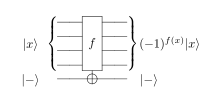
\includegraphics[scale=1]{fig05.02.png}
     \caption{The Oracle}
     \label{Fig:5.2}
   \end{minipage}
\end{figure}

\subsubsection*{Implementation of the Diffuser}
The diffuser has the equation as per equation \ref{eq:5.3}. To implement the diffuser on the state $\ket{000\cdots0}$, we just need to flip all qubits using $X$ gates and then apply a multi-controlled $Z$-gate. Since we are starting with the state $\ket{+++\cdots+}$, we need to apply a $H$-gate in the beginning and at the end to got to $\ket{000\cdots0}$ and revert back. Figure \ref{Fig:5.3} shows the diffuser circuit for 8 qubits.
\begin{figure}[!htb]
   \begin{minipage}{\textwidth}
     \centering
     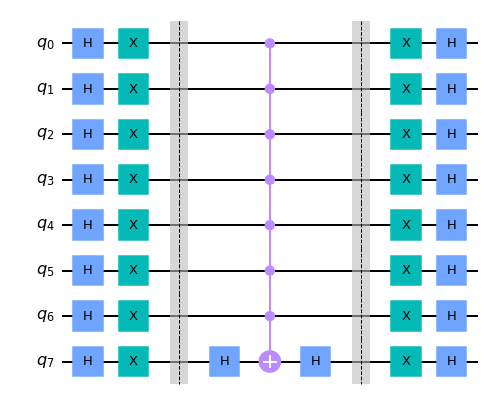
\includegraphics[scale=0.7]{fig05.03.png}
     \caption{The Diffuser for 8 qubits}
     \label{Fig:5.3}
   \end{minipage}
\end{figure}

\subsection{Number of Iterations}
Let our register consist of $n$ qubits. The number of pure states possible is then $2^n=N$. Consider the initial state of the system, where the system is initialized to $\ket{+++\cdots+}$. This is nothing but an equal superposition of the $N$ pure states. Since $\ket{\omega}$ is one of these states and all states occur with equal probabilities, probability of finding $\ket{\omega}$ is $\bfrac{1}{N}=\bfrac{1}{2^n}$. Now, from equation \ref{eq:5.4}, the probability of measuring $\ket{\omega}$ is $\sin^2\theta$. Thus we have,
\begin{equation}
\label{eq:5.8}
\begin{split}
\sin^2\theta&=\bfrac{1}{2^n}\\
\Rightarrow \sin\theta&=\sqrt{\bfrac{1}{2^n}}\\
\end{split}
\end{equation}
At each iteration we reflect by 2$\theta$. Thus, after $k$ iterations, we arrive at angle 2$k\theta$. For complete search, 2$k\theta$ should be as close as possible to $\bfrac{\pi}{2}$ but less than that (to avoid overshoot). For small $theta$, $\sin\theta\approx\theta$. Thus, we have
\begin{equation}
\label{eq:5.9}
\begin{split}
2k\theta&=\bfrac{\pi}{2}\\
\Rightarrow k\sqrt{\bfrac{1}{2^n}}&=\bfrac{\pi}{4}\\
\Rightarrow k&=\bfrac{\pi}{4}\sqrt{2^n}\\
\Rightarrow k&=\bfrac{\pi}{4}\sqrt{N}
\end{split}
\end{equation}
Thus, our complexity of search is $\mathcal{O}(\sqrt{N})$ as compared to $\mathcal{O}(N)$ for a classical brute force method. Further, if there are $M$ solutions instead of one and we are interested in finding at least one solution, the complexity of Grover's algorithm is $\mathcal{O}\left(\sqrt{\bfrac{N}{M}}\right)$.


\subsection{Generalized Grover Search}
Generalized Grover search\cite{gengrov} dwells on the main Grover Search algorithm, except that it reduces the number of gates required by using suitable alternate unitary gates. This further increases the efficiency of the algorithm.\\
The original grover iterate takes the form $G=OAM_0A\dagger$, where $A$ is any unitary operator (we have used the Hadamard) and $O$ is the oracle. The $M_0$ represents the mirroring circuit. $M_0$ has the form $M_0=X^{\otimes n}M_1X^{\otimes n}$, where $M_1$ is the mirror flip of the last bit implemented using the multi-controlled $Z$-gate. Thus, we have $G=OAM_0A\dagger=OAX^{\otimes n}M_1X^{\otimes n}A\dagger$. Setting $B=AX^{\otimes n}$ gives $B\dagger=X^{\otimes n}A\dagger$ since $X^{\otimes n}\dagger=X^{\otimes n}$.We can then write $G=OBM_1B\dagger$, where $M_1$ is a single gate and $B$ avoids the use of $=X^{\otimes n}$, thereby reducing the total number of gates.